\usetikzlibrary{shapes,arrows,positioning}

\tikzstyle{input} = [coordinate]
\tikzstyle{output} = [coordinate]
\tikzstyle{block} = [draw,rectangle]
\tikzstyle{sum} = [draw,circle]
\tikzstyle{gain} = [draw,isosceles triangle]

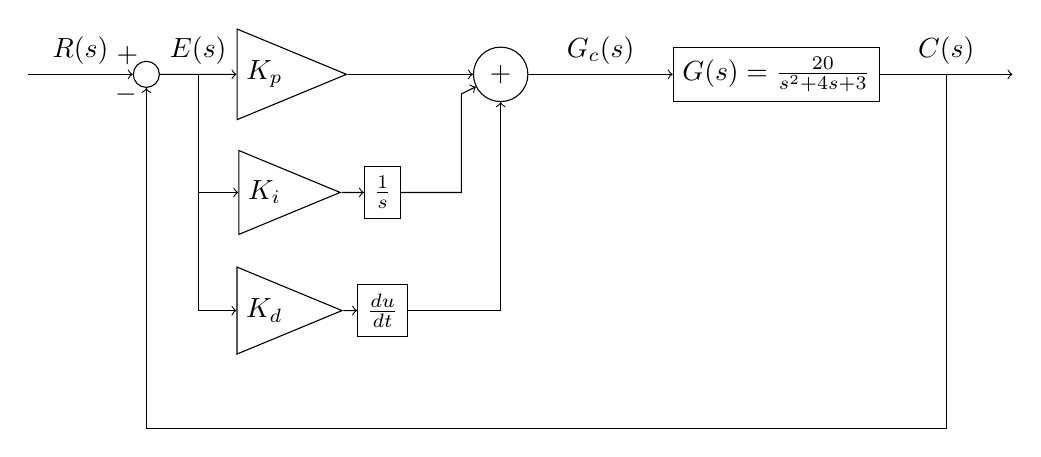
\begin{tikzpicture}[auto,node distance=1.5cm]
  \node[input] (in) {};
  %sum1
  \node[sum,right of=in] (sum1) {};

  %KP
  \node[gain,right of=sum1] (kp) {$K_p$};

  %KI
  \node[gain,below of=kp] (ki) {$K_i$};
  \node[block,right of=ki] (integrator) {$\frac{1}{s}$};

  %KD
  \node[gain,below of=ki] (kd) {$K_d$};
  \node[block,right of=kd] (derivative) {$\frac{du}{dt}$};

  %sum2
  \node[coordinate,right of=integrator] (p1) {};
  \node[sum,above of=p1] (sum2) {$+$};
  \node[draw,coordinate,left of=sum2,node distance=0.5cm] (ps21) {};
  \node[draw,coordinate,below of=ps21,node distance=0.25cm] (ps22) {};

  %plant
  \node[block,right of=sum2,node distance=3.5cm] (plant) {$G(s) = \frac{20}{s^2+4s+3}$};

  \node[output,right of=plant,node distance=3cm] (out) {};

  %draw the arrows
  \draw [->] (in) -- node {$R(s)$} node[pos=0.95] {+} (sum1);
  \draw [->] (sum1) -- node[name=p2]{$E(s)$} (kp);
  %PID arrows
  \draw [->] (kp) -- (sum2);
  \draw [->] (p2) |- (ki);
  \draw [->] (ki) -- (integrator);
  \draw [->] (integrator) -| (ps22) -- (sum2);
  \draw [->] (p2) |- (kd);
  \draw [->] (kd) -- (derivative);
  \draw [->] (derivative) -| (sum2);

  \draw [->] (sum2) -- node{$G_c(s)$} (plant);
  \draw [->] (plant) -- node[name=p3]{$C(s)$} (out);

  %feedback
  \node[coordinate,below of=derivative] (p4) {};
  \draw [->] (p3) |- (p4) -| node[pos=0.99]{$-$} (sum1);

\end{tikzpicture} 
